\cotefile{33}
\scanpage{171}
% archive sheet number: 170
\uline{Réédition des E. V. T.}, \uline{chap. II} \mspage{(7)}\hfill Tribu n° 63

l. 7, remplacer $V_\alpha$ par $g_\alpha(V_\alpha)$ ).

P. 55, vider les l. 1-8 du bas.

P. 56, vider les l. 1-2, et 1-12 du bas.

P. 57, l. 1 : II. Limites inductives d'espaces localement convexes. Se donner les $E_\alpha\subset E$ filtrants croissants avec $\bigcup E_\alpha=E$, avec les $E_\beta\to E_\alpha$ continues.

Vider les l. 9-14.

l. 13 du bas : Exemple.

P. 58, l. 1, vider 1).

Vider les l. 1-13 du bas.

P. 59, après la déf. 2, donner les voisinages de $0$.

(l. 1-8 du bas ; l. 8 du bas, attention au style).

Puis, dire que, pour tout $F$ localement convexe, on a $\mathscr{L}(E,F)=\prod\mathscr{L}(E_i,F)$, et que ceci caractérise la somme directe.

Corollaire : Une \uline{limi}te inductive est quotient d'une somme directe.

Proposition 6. L'injection canonique de $E$ dans $\prod E_i$ est continue. Si $I$ est fini, c'est un isomorphisme d'E. V. T.

P. 60, vider les l. 1-13 du bas.

P. 61, vider les l. 1-5.

Corollaire 1 (ex. 2) : Si les $G_i$ sont fermés, $\sum G_i$ est fermé.

Démonstration : $p_\alpha:E\to E_\alpha$ est continu, donc $p_\alpha^{-1}(G_\alpha)$ est fermé, donc $\bigcap p_\alpha^{-1}(G_\alpha)=\sum G_\alpha$ est fermé.

Vider les p. 62, 63, 64 (l. 1-4). On annoncera quelque part qu'une somme directe de complets est complète, mais on le démontrera plus tard à l'aide du th. de Grothendieck.

P. 64, le cor. 1 disparaît, puisqu'il a été glorifié tout de suite après la déf. des sommes directes. Le cor. 2 sera bloqué avec la prop. 7 (dont on conservera les notations), et sera à peu près évident sur la définition catégorique des sommes directes.

Vider la Remarque 2.

P. 65, l. 12, il faut pouvoir dire que $E$ est la limite inductive des $E_n$.

Annoncer : Dans tout le n°, $E$ sera la limite inductive des $E_n$.
\scanpage{172}
% archive sheet number: 171
% slanted
\margin{Généraliser \unsure{à|:} \unsure{des faisceaux|aux faisceaux} d'anneaux plus généraux}
\uline{Théorème} \inserted{\uline{à vérifier} !} Soit $X$ \inserted{\unsure{loc|loc.|lisse}} de type fini sur le corps $k$, $\dim X\leq n$ $A=Z/NZ$ $N$ premier à car. $k$, \deleted{\unsure{$A$|$A$-}} \inserted{$F$ et} $\unsure{G|C}$ deux $A$-\deleted{\unsure{faisc.|d'Alg.}}Modules. Supposons que $F$ soit plat \unsure{\uline{ou}|$=$} $G$ à fibres injectives ($=$ plates, dans le cas particulier envisagé !). Alors

(i) Si $F$ constructible, alors $\mathscr{E}xt^i(F,G)=0$ pour $i>2n$.

(ii) Si $k$ est séparablement clos, alors, \deleted{\unsure{pour tout|pour tout $i$|pareillement}}

\[
\begin{aligned}
\mathrm{Ext}^i(\unsure{X;|X,|A;|A,}F,G)&=0 &&\text{pour } i>\unsure{2|1|\,}n\\
\mathrm{Ext}^i(F,G)&=0 &&\text{pour } i>2n.
\end{aligned}
\]

\uline{Dém.} (i) se ramène par passage \unsure{à|:} la limite \unsure{à|:} (ii). Dans (ii) on peut supposer $k$ sép. clos, et \deleted{un argument général} il suffit de prouver la \uline{première} relation. \inserted{Supposer d'abord $G$ à fibres injectives.} Un argument général nous ramène à \deleted{\unsure{le|la|$G$}} vérifier \inserted{la formule} lorsque $F$ est quotient d'un \unsure{générateur|puissance|partie} de la forme $i_!(A_{X'})$, où $X'$ affine et $X'\unsure{-|\to}X$ étale, au dessus d'un ouvert affine \inserted{$U$} de $X$. \unsure{Cela|Ceci|Car} nous ramène au cas où $X=U$ est aussi affine [car on peut remplacer $X$ par $U$, $G$ par $G|U$]
\scanpage{173}
% archive sheet number: 172
\mspage{12}
\uline{Proof}. Follows from [A7, Lemma 3.19 of Section 14].

LEMMA 2. Let $(R,M)$ and $(\bar R,\bar M)$ be two regular local domains of the same dimension $n$ with quotient fields $K$ and $\bar K$ respectively. Assume that $K$ is a subfield of $\bar K$, $\bar R$ has center $M$ in $R$ and $M\bar R=\bar M$. Then $R/M$ can be canonically identified with a subfield of $\bar R/\bar M$; assume that under this identification $\bar R/\bar M=R/M$, i.e., given $x$ in $\bar R$ there exists $y$ in $R$ such that $x-y$ is in $\bar M$. Then given $x$ in $R$ and a positive integer $q$ there exists $y$ in $R$ such that $x-y$ is in $\bar M^q$. Also we have that $K\handwritten{\cap}\bar R=R$, $K\handwritten{\cap}\bar M=M$, $M^qR=\bar M^q$ for any positive integer $q$, and if $A$ is any ideal in $R$ then $(A\bar R)\handwritten{\cap}R=A$ and $A$ is principal if and only if $A\bar R$ is principal, in particular $\bar M^q\handwritten{\cap}R=M^q$ for any positive integer $q$. Consequently, any completion of $\bar R$ is also a completion of $R$.

\uline{Proof}. From $M\bar R=\bar M$ we at once have $M^q\bar R=\bar M^q$ for all $q>0$. By induction on $q$ we shall show that given $x$ in $\bar R$ there exists $y$ in $R$ such that if $x-y$ is in $\bar M^q$; for $q=1$ this is given, so assume that $q>1$ and that this is true for $q-1$. Then given $x$ in $\bar R$ there exists $z$ in $R$ such that $x-z$ is in $\bar M^{q-1}$; since $\bar M^{q-1}=M^{q-1}R$, $x-z=\sum a_i b_i$ with $a_i$ in $M^{q-1}$ and $b_i$ in $\bar R$, the assumption for $q=1$ tells us that there exists $c_i$ in $R$ and $d_i$ in $\bar M$ such that $b_i=c_i+d_i$, let $y=z+\sum a_i c_i$, then $x-y=\sum a_i d_i$ which is in $\bar M^q$.

Now let $x_1,\ldots,x_n$ be a minimal basis of $M$, since $M\bar R=\bar M$
\scanpage{174}
% archive sheet number: 173
et $F$ constructible. De plus, par passage à la limite on peut supposer \unsure{alors} $\unsure{G|C}$ également constructible [Attention, est-il vrai que $G$ est limite ind. \margin{?}\inserted{\uline{\unsure{filtrante|filtrant}}} des \deleted{\unsure{sous|ses|tous}} faisceaux const. à fibres \uline{injectives} ?? ].
\scanpage{175}
% archive sheet number: 174
\mspage{11}
and by $f^{-1}(W)$ we shall denote as usual the set theoretic inverse image of the set of points of $W$. \unsure{It.|It} can be immediately verified that if $W$ is irreducible and of co-dimension one so that $Q(W,V)$ is the valuation ring of a real discrete valuation $v$ of $K(V)/k$ then $f^{-1}[W]$ is also irreducible of co-dimension one and it is the center of $v$ on $V^*$.

2. \uline{Auxiliary Lemmas}.

LEMMA 1. Let $(R,M)$ be a regular local domain of dimension $n>1$ with quotient field $K$. Let $x_1,\ldots,x_n$ be a minimal basis of $M$. Let $y_1=x_1$, $\deleted{y_i=x_i\vert\alpha_1}\handwritten{\inserted{y_i=x_i/x_1}}$ for $i=2,\ldots,n$ and let $S=R[y_2,\ldots,y_n]$. Then we have $(y_1S)\handwritten{\cap}R=M$ so that $R/M$ can be canonically identified with a subfield of $S/(y_1S)$ and then the residues $\bar y_2,\ldots,\bar y_n$ respectively of $y_2,\ldots,y_n$ modulo $y_1S$ are algebraically independent over $R/M$ and hence $S/(y_1S)$ can be identified with the polynomial ring $(R/M)[\bar y_2,\ldots,\bar y_n]$ in $n-1$ variables. Then the canonical homomorphism of $S$ onto $S/(y_1S)$ sets up a one to one correspondence between the maximal ideals in $S$ containing $y_1$ and the maximal ideals in the polynomial ring $S/(y_1S)$, and hence if $P$ is a maximal ideal in $S$ containing $y_1$ and $R_1=S_P\handwritten{\subset} K$ and $M_1=PR_1$ then $(R_1,M_1)$ is a regular local domain of dimension $n$ having center $M$ in $R$, $y_1$ is part of a minimal basis of $M_1$ and $R_1/M_1$ is a finite algebraic extension of $R/M$.
\scanpage{176}
% archive sheet number: 175
\[
\mathscr{E}xt^p(F,G)
\]

\[
\mathscr{E}xt^{\unsure{p|q|n}}(i_!(F),G)\simeq
\unsure{\mathscr{E}|\mathrm E}xt^p(F,\mathbb R i^!(G))
\]

\[
\mathscr{E}xt^*(F,\mathbb R i^!(G))\unsure{\Leftarrow|\ne|=}E_2^{pq}=\mathscr{E}xt^p(F,\mathbb R^qi^!(G))
\]

\diagram{\begin{tikzcd}[ampersand replacement=\&,column sep=0.4em]
Y \& \unsure{\longleftrightarrow|\longleftarrow|\hookrightarrow} \& X
\end{tikzcd}}

\[
\mathscr{E}xt^p(F,\underset{\rule{.5pt}{.4em}\rule{3em}{.5pt}\rule{.5pt}{.4em}}{\mathbb R^qi^!G})
\]

\[
\mathscr{E}xt^p
\]

\figure{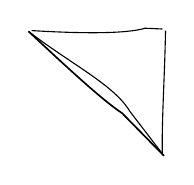
\begin{tikzpicture}[x=1cm,y=1cm]
\draw (0.04,1.59) .. controls (.7,1.55) and (1.25,1.55) .. (1.48,1.62) -- (1.70,1.61);
\draw (1.74,1.59) .. controls (1.73,1.0) and (1.69,.45) .. (1.70,.01);
\draw[semithick] (0,1.58) .. controls (.45,1.16) and (.92,.72) .. (1.19,.54) -- (1.72,0);
\draw (0,1.58) .. controls (.53,1.17) and (1.09,.90) .. (1.29,.56) -- (1.72,0);
\end{tikzpicture}}

\diagram{\scriptsize\setlength{\arraycolsep}{1.6pt}
$\begin{array}{c@{}c@{\;}c@{}c@{}c@{\quad}c@{}c@{\quad}c@{}cc}
\unsure{\leq d|2d} & & \leq d-1 & & \leq d-2 & & & & 0 &\\
\mathscr{E}xt^0, & \mathscr{E}xt^1 & \mathscr{E}xt^2 & / &
\mathscr{E}xt^3\;\mathscr{E}xt^4 & / & & / & \mathscr{E}xt^{2d-1}, & \mathscr{E}xt^{2d}
\end{array}$}

\[
H^p(X,\mathscr{E}xt^q\qquad
\deleted{H^{\unsure{n|q}}}\ H^{\unsure{n|2d}}(X,\mathscr{E}xt^0)+H^{n-1}\mathscr{E}xt^1,\ \unsure{.|\,}
\]

\figure{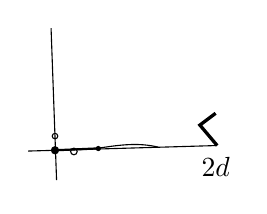
\begin{tikzpicture}[x=1cm,y=1cm]
\draw (-.05,1.55) -- (.02,-.38);
\draw (-.34,-.01) -- (2.05,.06);
\draw[thick] (0,0) -- (.58,.025);
\draw (.54,.025) .. controls (.83,.07) and (1.06,.10) .. (1.31,.04);
\fill (0,0) circle (1.5pt); \draw (.0,.18) circle (1pt); \draw (.24,-.015) circle (1.2pt);
\fill (.55,.022) circle (.95pt);
\draw[very thick] (2.06,.06) -- (1.84,.32) -- (2.04,.47);
\node[below] at (2.04,.04) {$2d$};
\end{tikzpicture}}

\[
p\leq \qquad
\begin{array}{ccc}
 & n-1\unsure{.|\,}\leq2(d-1)&n-3\leq2(d-2)\\
n\leq2d & \deleted{\unsure{n-1|n+1}\leq2d-1}&\\
 & n-2\leq2(d-1)&n-4\leq2(d-2)
\end{array}
\]

\[
\deleted{\mathrm{Ext}^*(F,G)\simeq}\qquad \underline{2d-1}
\]

\figure{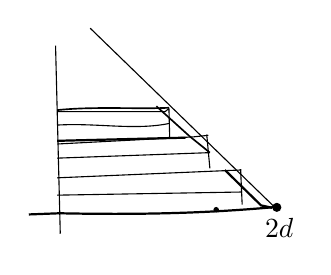
\begin{tikzpicture}[x=1cm,y=1cm]
\draw (-.02,2.13) -- (.04,-.26);
\draw[thick] (-.36,-.015) -- (.03,0) .. controls (1.25,-.025) and (2.06,.015) .. (2.78,.08);
\draw (.42,2.35) -- (2.76,.08);
\draw[semithick] (.0,1.31) .. controls (.47,1.36) and (1.03,1.32) .. (1.42,1.34);
\draw (.00,1.29) -- (1.37,1.29) -- (1.42,1.33) -- (1.43,.95);
\draw (.0,1.12) .. controls (.51,1.15) and (.98,1.05) .. (1.42,1.14);
\draw[thick] (.0,.92) -- (1.63,.96); \draw (.01,.88) -- (1.73,.97) -- (1.92,.99);
\draw (.0,.70) -- (1.94,.77); \draw (1.90,1) -- (1.94,.57);
\draw (.0,.45) -- (2.34,.55); \draw (2.33,.56) -- (2.35,.11);
\draw (.0,.23) -- (2.35,.27);
\draw[semithick] (1.26,1.36) -- (1.68,.98) -- (1.94,.77);
\draw[thick] (2.13,.55) -- (2.59,.10) -- (2.73,.07);
\fill (2.02,.045) circle (1pt); \fill (2.79,.075) circle (1.65pt);
\node[below] at (2.82,.06) {$2d$};
\end{tikzpicture}}

\[
\mathbb R\mathscr{H}om(F,\deleted{\unsure{D|G}}G)\simeq
\mathbb R\mathscr{H}om(F\otimes DG,K_X)
\]

\[
\mathrm{Ext}^{p+q}(X;F,G)\Leftarrow E_2^{pq}=\mathrm{Ext}^p(X;\mathrm{Ext}^{-q}(X;G,A_X),A_X)
\]

\[
\mathrm{Ext}^{2d}(X;F,G)
\]

\figure{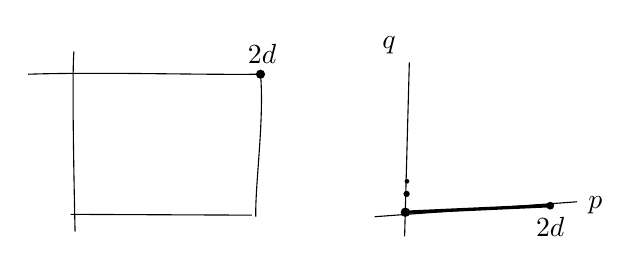
\begin{tikzpicture}[x=1cm,y=1cm]
\draw (0,2.12) .. controls (-.025,1.81) and (.0,.49) .. (.015,-.17);
\draw (-.58,1.83) .. controls (.35,1.86) and (1.57,1.82) .. (2.37,1.83);
\draw (2.37,1.83) .. controls (2.42,1.26) and (2.30,.43) .. (2.31,.02);
\draw (-.04,.05) -- (2.26,.04); \fill (2.37,1.83) circle (1.65pt);
\node[above] at (2.39,1.84) {$2d$};
\begin{scope}[xshift=4.2cm]
\draw (.06,1.98) -- (0,-.23); \draw (-.38,.02) -- (2.19,.21);
\draw[very thick] (.01,.077) -- (1.85,.16); \fill (.01,.077) circle (1.7pt);
\fill (.025,.31) circle (1.15pt); \fill (.03,.47) circle (.85pt); \fill (1.85,.16) circle (1.4pt);
\node[above left] at (.01,1.96) {$q$}; \node[right] at (2.21,.16) {$p$}; \node[below] at (1.85,.135) {$2d$};
\end{scope}
\end{tikzpicture}}

\[
\mathrm{Ext}^*(X;F,A_X)\Leftarrow \deleted{\unsure{E|H}}H^p(X,\mathscr{E}xt^q(F,A_X))\qquad{}^{2(d}
\]

\[
H^{2d}(X,
\]

\figure{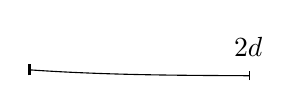
\begin{tikzpicture}[x=1cm,y=1cm]
\draw (0,0) .. controls (1,-.07) and (2,-.07) .. (2.80,-.075);
\draw[very thick] (0,-.07) -- (0,.07); \draw (2.8,-.13) -- (2.8,-.01);
\node[above] at (2.78,.05) {$2d$};
\end{tikzpicture}}
\scanpage{177}
% archive sheet number: 176
\mspage{67}
Note that $C_n^v$ is an even function for $n$ even and an odd function for $n$ odd, hence we have

\[
\handwritten{\gamma_{\unsure{m|n}}}=\handwritten{\left\{}
\begin{aligned}
&\frac{w_p}{C_n^{1/2\,p}(1)}\,i\pi\handwritten{\int}\limits_0^1 C^{1/2\,p}(x)(1-x^2)^{1/2\,p-1/2}\,dx && n\text{ odd}\\[4pt]
-&\frac{2w_p}{C_n^{1/2\,p}(1)}\handwritten{\int}\limits_0^1\log x\ C_n^{1/2\,p}(x)(1-x^2)^{1/2\,p-1/2}\,dx && n\text{ even}
\end{aligned}\right.
\]

the result is then proved by evaluating these integrals (see [18a]).

\uline{4.5\quad Reduction of a singular equation to the Fredholm case}.

We now return to the algebra $\handwritten{\mathscr{G}}$ of singular operators on $M$. For each $J\in\handwritten{\mathscr{G}}$ and each $x\in M$ we shall define the symbol of $J$ at $x$; this will be a function on $S_x$. Let $\mathbb{H}_xJ$ be the homogeneous part of $J$ at $x$; we define $\mathbb{S}_xJ=\mathbb{S}\mathbb{H}_xJ$, thus $\mathbb{S}_x$ is the composition of the homomorphism $\mathbb{H}_x$ and the isomorphism $\mathbb{S}$.

\uline{Definition 4.5.1.}\qquad If $J\in\handwritten{\mathscr{G}}$ then the \uline{global symbol} of $J$ is a function on the tangent sphere bundle $S(M)$ defined by

\[
\mathbb{S}_M J(b)=\mathbb{S}_{\pi(b)}J(b).
\]

Note that $\mathbb{S}_M J=0$ implies that $\mathbb{H}_x J=0$ for all $x\in M$ and $J\in\handwritten{\bigcap}\limits_{x\in M}\handwritten{\mathscr{F}}_x=\handwritten{\mathscr{F}}$, so $J$ is completely continuous.
\scanpage{178}
% archive sheet number: 177
\figure{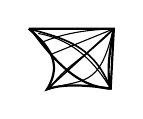
\begin{tikzpicture}[x=1cm,y=1cm]
\draw[thick] (0,.78) -- (1.08,.78) -- (1.04,.02) .. controls (.77,.06) and (.44,.09) .. (.23,.01)
 .. controls (.46,.37) and (.20,.61) .. (0,.78);
\draw[semithick] (0,.78) .. controls (.49,.65) and (.83,.55) .. (1.04,.02);
\draw[thick] (.03,.77) .. controls (.34,.35) and (.63,.04) .. (1.04,.02);
\draw (.12,.72) .. controls (.59,.64) and (.86,.32) .. (1.04,.02);
\draw (.17,.61) .. controls (.46,.73) and (.77,.77) .. (1.08,.78);
\draw (.27,.45) -- (1.08,.78); \draw[semithick] (.23,.01) -- (1.08,.78);
\draw (.26,.01) .. controls (.43,.29) and (.72,.41) .. (1.08,.78);
\draw (.23,.01) .. controls (.69,.15) and (.90,.02) .. (1.07,.77);
\draw[thick] (1.04,.02) .. controls (.97,.27) and (1.06,.65) .. (1.08,.78);
\end{tikzpicture}}

\[
\mathscr{E}xt^i(F,G)
\]

\[
\unsure{F_2|F_\ell|\deleted{F}}\qquad DG
\]

\[
\begin{aligned}
\mathbb R\mathscr{H}om(F,G)&\unsure{=|\simeq}\mathbb R\mathscr{H}om(F,DDG)\\
&\simeq\mathbb R\mathscr{H}om(F_{\unsure{,|1|\,}}\overset{\mathbb L}{\otimes}DG,R_X^\bullet)
\end{aligned}
\]

\[
F_{\unsure{1|<|\,}}\otimes DG
\]

\figure{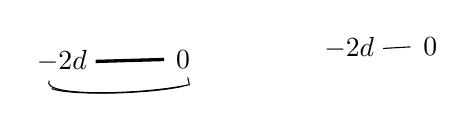
\begin{tikzpicture}[x=1cm,y=1cm]
\node at (0,0) {$-2d$}; \draw[very thick] (.43,-.005) -- (1.30,.02); \node at (1.54,.02) {$0$};
\draw (-.16,-.25) .. controls (-.27,-.46) and (1.03,-.43) .. (1.62,-.30) -- (1.60,-.21);
\draw (-.13,-.35) .. controls (.11,-.44) and (1.08,-.42) .. (1.54,-.32);
\node at (3.65,.17) {$-2d$}; \draw (4.08,.16) -- (4.43,.18); \node at (4.68,.18) {$0$};
\end{tikzpicture}}

\[
\deleted{\mathscr{E}xt^{i}}\qquad\mathscr H_i(F\otimes DG)\qquad\text{de }\dim\leq i
\]

\[
\mathscr{E}xt^i(F,G)\qquad D(F\overset{\mathbb L}{\otimes}DG
\]

\[
\boxed{\mathrm{Ext}^{\unsure{+|*}}(F_{\unsure{1|,|\,}},G)\Leftarrow E_1^{pq}=\mathrm{Ext}^{p\deleted{\unsure{+q|-q}}}(F\otimes\mathscr{E}xt^{-q}(G,A_X),A_X)}
\]

\figure{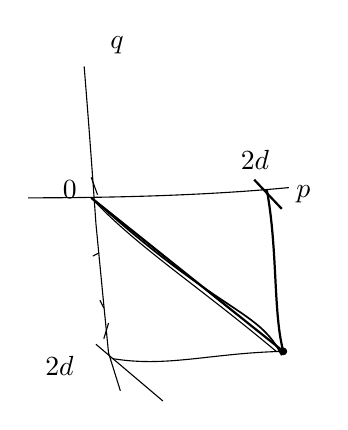
\begin{tikzpicture}[x=1cm,y=1cm]
\draw (-.8,0) .. controls (.10,0) and (1.36,.02) .. (2.51,.13);
\draw (-.09,1.67) .. controls (-.03,.94) and (.03,.10) .. (.06,-.33)
 -- (.15,-1.26) -- (.22,-1.97) -- (.37,-2.45);
\draw[thick] (2.23,.10) .. controls (2.37,-.65) and (2.31,-1.48) .. (2.44,-1.95);
\draw (.26,-2.04) .. controls (.96,-2.16) and (1.52,-1.97) .. (2.44,-1.95);
\draw[thick] (0,0) -- (2.44,-1.95);
\draw (0,0) .. controls (.58,-.62) and (1.31,-1.08) .. (2.35,-1.95);
\draw[semithick] (.04,-.03) .. controls (1.68,-1.50) and (2.12,-1.41) .. (2.42,-2);
\draw (0,.26) -- (.08,.04); \draw (.02,-.74) -- (.1,-.70);
\draw (.16,-1.40) -- (.11,-1.30); \draw (.16,-1.79) -- (.22,-1.59);
\draw (.06,-1.86) -- (.91,-2.58);
\draw[thick] (2.07,.23) -- (2.42,-.14); \fill (2.44,-1.95) circle (1.4pt);
\node[above right] at (.12,1.7) {$q$}; \node[left] at (-.06,.11) {$0$};
\node[above] at (2.08,.24) {$2d$}; \node[right] at (2.48,.04) {$p$};
\node[left] at (-.10,-2.13) {$2d$};
\end{tikzpicture}}

\[
\deleted{\unsure{q^4-q|q^4-q^1|q^4=q}}\unsure{2q|\geq q}\qquad F\otimes\mathscr{E}xt^{2d}(G,A)
\]

\[
\deleted{\mathscr{E}xt^p(}
\]

$\operatorname{supp}\mathscr{E}xt^{-q}(G,A_X)$ de \deleted{\unsure{d|D}}codim $\geq-q$

\deleted{de dim $\leq$}

donc $\mathscr{E}xt^p(\ ,A_X)=0$ si $p\unsure{<|\leq}-q$ i.e. si $\unsure{pq|p+q}<0$

\[
\deleted{\mathscr{E}xt^*(}\qquad \mathscr{E}xt^{2d}(F,G)\simeq\mathscr{E}xt^{2d}(F\otimes\mathscr{H}om(G,A_X),A_X)
\]
\scanpage{179}
% archive sheet number: 178
\mspage{68}
Let $\handwritten{\mathscr{S}}_M$ be the algebra of $C^\infty$ functions on $S(M)$; then:

\uline{Theorem 4.5.2.}\qquad The map $\mathbb{S}_M:\handwritten{\mathscr{G}\longrightarrow\mathscr{S}}_M$ is an epimorphism whose kernel is $\handwritten{\mathscr{F}}$, the ideal of completely continuous operators.

Our problem now is to ``regularize'' the equation

\begingroup
\csname tagsleft@true\endcsname
\[
J\handwritten{\rho}=f\tag*{(4.5.3)}
\]
\endgroup

that is to reduce it to an equation of Fredholm type. We wish to find an operator $K\in\handwritten{\mathscr{G}}$ such that the equation $KJ\handwritten{\rho}=Kf$ is of Fredholm type and has the same solutions as the original equation.

Now, if $KJ=Kf$ is of Fredholm type this means that $KJ=I+L$ where $L\in\handwritten{\mathscr{F}}$ and then $\mathbb{S}_M KJ=1$. Hence a necessary condition for the existence of a reduction is $\mathbb{S}_M J(b)\handwritten{\not}=0$ for all $b\in S(M)$. This condition is also sufficient:

\uline{Theorem 4.5.4.}\qquad If $J\in\handwritten{\mathscr{G}}$ then the equation $J\handwritten{\rho}=f$ can be regularized if and only if $\mathbb{S}_M J(u)\handwritten{\not}=0$ for all $u\in S(M)$.

\uline{Proof:}\quad We must find an operator $K\in\handwritten{\mathscr{G}}$ such that $KL=Kf$ has the same solutions as (4.5.3) and is of Fredholm type. Let $K_1$ be any operator such that $\mathbb{S}_M K_1\cdot\mathbb{S}_M J=1$; then clearly:
\scanpage{180}

\diagram{\scriptsize
\begin{tikzcd}[ampersand replacement=\&,column sep=small,row sep=3pt,execute at end picture={
\node[align=left,anchor=north] (noteone) at ([xshift=-.5em,yshift=-.9em]aone.south) {dualité\\parfaite\\\unsure{trivialement|triviale}\\(via \unsure{poncti\ldots|ponctu\ldots|pureté\ldots})};
\node[align=left,anchor=north] (notetwo) at ($(atwo.south)!.5!(athree.south)+(0,-2.3em)$) {dualité\\parfaite ??};
\draw[thin] ([xshift=-.6em,yshift=.8em]aone.north) to[bend right=22] ([xshift=-.35em]noteone.north);
\draw ([xshift=.5em,yshift=1em]atwo.north) to[bend left=24] ([xshift=-.5em]notetwo.north);
\draw[thin] ([xshift=-.5em,yshift=.8em]athree.north) to[bend right=6] ([xshift=.35em]notetwo.north);
}]
\cdots \arrow[r,dash] \& \mathbb R^i\Gamma_x(F) \arrow[r] \& \mathbb R^i\Gamma_X(F) \arrow[r] \& \mathbb R^i\Gamma_U(F) \arrow[r,dash] \& \mathbb R^{i+1}\Gamma_x(F) \arrow[r,dash] \& \cdots \\
\& \& \times \& \times \& \times \& \\
\& \mathbb R^{-i}\Gamma_X(DF) \& \mathbb R^{-i}\Gamma_x DF \arrow[l] \arrow[d] \& \mathbb R^{-i}\Gamma_U(F) \arrow[l] \arrow[d] \& \mathbb R^{-i-1}\Gamma_X DF \arrow[l] \arrow[d,dash] \& \cdots \arrow[l] \\
\& \& |[alias=aone]| A \& |[alias=atwo]| A \& |[alias=athree]| A \&
\end{tikzcd}}

\[
\begin{aligned}
f^!\mathbb R\mathscr H\!om(\unsure{F^\bullet|f^\bullet|F},G^\bullet)\\
f^!D=Df^*
\end{aligned}
\]

\[
\begin{aligned}
\deleted{\unsure{D|R}}\mathbb R\mathscr H\!om(F,G)\\
D(F\otimes DG)\\[3pt]
\mathbb R\mathscr H\!om(G,DF)\\
=D(G\overset{\mathbb L}{\otimes}F)\\
\mathbb R\unsure{\mathscr H\!om|\mathscr H}(F,D(DG))\\
\mathbb R\unsure{\mathscr H|\mathscr H\!om}
\end{aligned}
\]

\[
D(H_x^i(F))\longrightarrow\deleted{\unsure{D(F|D(DF|D}}\to
\mathscr H_{\unsure{x|\,}}^{i}\bigl(DF\bigr)_x\unsure{\bigr\}|)}
\]

\[
\begin{aligned}
F&\longrightarrow DDF\\
\deleted{H_x^i(F)\longrightarrow}&\\
\mathscr H^{i}(F)_x&\unsure{-|\to}D_x\underset{\rule{.4pt}{.32em}\rule{4.1em}{.4pt}\rule{.4pt}{.32em}}{\mathscr H_x^{-i}(D_XF)}\\
& D_x\deleted{\unsure{\mathscr H|D}}D_x(\mathscr H^i(F)_x)
\end{aligned}
\]

\[
D(F\otimes DG)=D\mathbb R\mathscr H\!om(F,\underset{D}{G})
\]

\figure{\begin{tikzpicture}[x=1cm,y=1cm]
\draw[very thick] (-2.9,.2)--(-2.65,.2)--(-2.65,-.24)--(-2.9,-.24);
\draw[very thick] (-1.78,.39)--(-2.05,.33)--(-2.05,-.12)--(-1.77,-.05);
\draw (-2.65,.05)--(-2.05,.13);
\node[anchor=east] at (-3.65,-.35) {$F\otimes DG$};
\node[anchor=east] at (-3.65,-.84) {$-2n,0$};
\draw[very thick] (1.25,1.28)--(1.44,1.3)--(1.44,1.02)--(1.25,.99);
\draw[very thick] (2.99,1.46)--(2.83,1.45)--(2.83,1.14)--(2.99,1.16);
\draw (1.44,1.14)--(2.83,1.31);
\node at (2.59,.62) {$F$};
\draw (2.96,.08)--(5.73,.39);
\draw (3.44,.10)--(3.44,.21) (5.4,.28)--(5.4,.47);
\fill (4.87,.29) circle (.025);
\node[below] at (3.44,.10) {$M$}; \node[below] at (4.87,.27) {\scriptsize $0$}; \node[below] at (5.4,.28) {$N$};
\draw (5.09,-.73)--(5.82,-.67); \draw (5.09,-.77)--(5.09,-.69) (5.82,-.72)--(5.82,-.62);
\node[below] at (5.21,-.73) {$-2n$};
\end{tikzpicture}}

\[
\begin{aligned}
&\text{Tor-dim}_{*}\,F_{\bullet}\quad\text{\unsure{majorée|majoré|concentrée} par}\quad[N,M]\\[-1pt]
\Downarrow\quad &\\
&\text{loc-Inj-dim}^{*}\ D(F)\quad\text{majorée par}\quad[-2n+N,M]\\
&\text{Inj-dim}\ F\quad\text{majorée par}\quad[P,Q]\\
\Downarrow\quad &\\
&\text{Tor-dim}\ DF\quad\text{majorée par}\quad[P-2n,Q]
\end{aligned}
\]

\[
\begin{aligned}
DF\overset{\mathbb L}{\otimes}G&=D\underset{\rule{.4pt}{.32em}\rule{6em}{.4pt}\rule{.4pt}{.32em}}{\mathbb R\mathscr H\!om(G,F)}\\
\deleted{DF\otimes DDG=D(F\otimes D}&\\
&[P,Q]\\
&-
\end{aligned}
\]
% archive sheet number: 179
\scanpage{181}
\mspage{24}

LEMMA 11. Let $(R^*,N^*)$ be a quadratic transform of $R$. Then there exists a unique integer $m$ such that $R^*$ is an $m$-th quadratic transform of $R$, also there exists a unique sequence $R=R_o,R_1,\ldots,R_m=R^*$ such that $R_i$ is an immediate quadratic transform of $R_{i-1}$ for $i=1,\ldots,m$. Furthermore $R_o,\ldots,R_m$ are the only quadratic transforms of $R$ which are contained in $R^*$. Also if $v$ is a valuation of $K$ having center $M^*$ in $R^*$ then $R_o,\ldots,R_m$ are the only $q$-th quadratic transforms of $R$ with $q\deleted{\unsure{<|\leq}}\handwritten{\inserted{\leq}}m$ which are contained in $R_v$ (it is obvious that in each of them $v$ has center at the maximal ideal).

\uline{Proof}. F\deleted{r}ollows from Lemmas 9 and 10 by induction.

DEFINITION 2. \uline{Let} $v$ \uline{be a valuation of} $K$ \uline{having center}\margin{\handwritten{\makebox[0pt][r]{\raisebox{-.62\height}[0pt][0pt]{$\left.\rule{0pt}{7\baselineskip}\right\}$}\,}Italicize only the underlined portion}} $M$ \uline{in} $R$ \uline{and of} $R$-\uline{dimension zero}. \uline{Then} by Lemma 11 above and [A6, Lemma 10] it follows that \uline{for each} $m$ \uline{there exists a unique} $m$-\uline{th quadratic transform} $(R_m,M_m)$ \uline{of} $R$ \uline{such that} $v$ \uline{has center} $M_m$ \uline{in} $R_m$; \uline{and then for all} $m$, $R_m$ \uline{is an immediate quadratic transform of} $R_{m-1}$ \uline{and the} $R_m$-\uline{dimension of} $v$ \uline{is zero}. \uline{We shall say that} $R_m$ \uline{is the} $m$-\uline{th quadratic transform of} $R$ \uline{along} $v$ \uline{and that} $R=R_o,R_1,R_2,\ldots$ \uline{is the quadratic sequence of} $R$ \uline{along} $v$.

LEMMA 12. Let\unsure{,} $(\bar R,\bar M)$ be an $n$-dimensional regular local domain such that the quotient field $\bar K$ of $\bar R$ contains $K$ as a subfield, $\bar R$ has center $M$ in $R$, $M\bar R=\bar M$ and
% archive sheet number: 180
